\documentclass[a4paper, 11pt, amsmath]{article}\usepackage[]{graphicx}\usepackage[]{color}
%% maxwidth is the original width if it is less than linewidth
%% otherwise use linewidth (to make sure the graphics do not exceed the margin)
\makeatletter
\def\maxwidth{ %
  \ifdim\Gin@nat@width>\linewidth
    \linewidth
  \else
    \Gin@nat@width
  \fi
}
\makeatother

\definecolor{fgcolor}{rgb}{0.345, 0.345, 0.345}
\newcommand{\hlnum}[1]{\textcolor[rgb]{0.686,0.059,0.569}{#1}}%
\newcommand{\hlstr}[1]{\textcolor[rgb]{0.192,0.494,0.8}{#1}}%
\newcommand{\hlcom}[1]{\textcolor[rgb]{0.678,0.584,0.686}{\textit{#1}}}%
\newcommand{\hlopt}[1]{\textcolor[rgb]{0,0,0}{#1}}%
\newcommand{\hlstd}[1]{\textcolor[rgb]{0.345,0.345,0.345}{#1}}%
\newcommand{\hlkwa}[1]{\textcolor[rgb]{0.161,0.373,0.58}{\textbf{#1}}}%
\newcommand{\hlkwb}[1]{\textcolor[rgb]{0.69,0.353,0.396}{#1}}%
\newcommand{\hlkwc}[1]{\textcolor[rgb]{0.333,0.667,0.333}{#1}}%
\newcommand{\hlkwd}[1]{\textcolor[rgb]{0.737,0.353,0.396}{\textbf{#1}}}%

\usepackage{framed}
\makeatletter
\newenvironment{kframe}{%
 \def\at@end@of@kframe{}%
 \ifinner\ifhmode%
  \def\at@end@of@kframe{\end{minipage}}%
  \begin{minipage}{\columnwidth}%
 \fi\fi%
 \def\FrameCommand##1{\hskip\@totalleftmargin \hskip-\fboxsep
 \colorbox{shadecolor}{##1}\hskip-\fboxsep
     % There is no \\@totalrightmargin, so:
     \hskip-\linewidth \hskip-\@totalleftmargin \hskip\columnwidth}%
 \MakeFramed {\advance\hsize-\width
   \@totalleftmargin\z@ \linewidth\hsize
   \@setminipage}}%
 {\par\unskip\endMakeFramed%
 \at@end@of@kframe}
\makeatother

\definecolor{shadecolor}{rgb}{.97, .97, .97}
\definecolor{messagecolor}{rgb}{0, 0, 0}
\definecolor{warningcolor}{rgb}{1, 0, 1}
\definecolor{errorcolor}{rgb}{1, 0, 0}
\newenvironment{knitrout}{}{} % an empty environment to be redefined in TeX

\usepackage{alltt}
% R vignette preable

\usepackage{amsmath}
\usepackage{mathtools}
\usepackage{amsfonts}
\usepackage{amssymb}
\usepackage{hyperref}

\usepackage{geometry}
 \geometry{
 a4paper,
 total={170mm,257mm},
 left=20mm,
 top=20mm,
 }
 
\usepackage{fancyhdr}
\pagestyle{fancy}
\renewcommand{\headrulewidth}{0pt}
\renewcommand{\footrulewidth}{0pt}
\setlength\headheight{80.0pt}
\addtolength{\textheight}{-80.0pt}
\lhead{
\includegraphics[width=0.34\textwidth]{UoLLogoMono.pdf}}

\def\bmu{{\mbox{\boldmath $\mu$}}}
\def\bs{{\mbox{\boldmath $\sigma$}}}
\def\bt{{\mbox{\boldmath $\theta$}}}
\IfFileExists{upquote.sty}{\usepackage{upquote}}{}
\begin{document}
\title{2. Simulating simple Gaussian Processes}
\author{Simon Vaughan \thanks{Email: sav2@le.ac.uk}}
\maketitle

%%%%%%%%%%%%%%%%%%%%%%%%%%%%%%%%%%%%%%%%%%%%%%%
\textbf{Details for generating Gaussian variables.} \\

How does a function like {\tt rmvnorm()} actually produce the Gaussian vector output with the right correlation structure?

We begin with $\mathbf{x} = ( x_1, x_2, \ldots, x_n )^T$ where all the $x_i$ are independently distributed with a Gaussian distribution, mean $\mu=0$ and variance $\sigma^2=1$ for all $i$. We can think of $\mathbf{x}$ as random vector with a Gaussian distribution, with mean vector $\bmu = 0$, and a simple covariance matrix $\Sigma = I_n$ where $I_n$ is the $n \times n$ identity matrix. 

\begin{equation}
 cov(\mathbf{x}) = E[(\mathbf{x}-\bmu)(\mathbf{x}-\bmu)^T] = E[\mathbf{x} \mathbf{x}^T] = I_n
\end{equation}

We wish to produce a vector $\mathbf{y} = (y_1, y_2, \ldots, y_n )^T$ which has the right covariance structure. To do this we left multiply the original random vector $\mathbf{x}$ by a matrix $L$ such that the output, $\mathbf{y}$, has the right covariance matrix. 

\begin{equation}
 \mathbf{y} = L \mathbf{x}
\end{equation}

The right matrix to chose is the Cholesky decomposition (the `matrix square root') of $S$, the covariance matrix. 

\begin{equation}
  S = L L^T
\end{equation}

$L$ is an $n \times n$ lower triangular matrix. Now, we can check the covariance of $\mathbf{y}$ is what we want

\begin{align}
  cov(\mathbf{y}) & = E[ \mathbf{y} \mathbf{y}^T  ]  \\
  \intertext{substituting $\mathbf{y} = L \mathbf{x}$ we get}
                  & = E[ (L \mathbf{x})  (L \mathbf{x})^T ]  \\
  \intertext{using $(L \mathbf{x})^T = \mathbf{x}^T L^T$ we get}
                  & = E[ L \mathbf{x} \mathbf{x}^T L^T ]   \\
  \intertext{The matrix $L$ is constant, so is just a constant factor on the expectation $E[\ldots]$}
                  & = L E[ \mathbf{x}  \mathbf{x}^T] L^T  \\
  \intertext{Now we notice that $E[ \mathbf{x}  \mathbf{x}^T] = I_n$, the covariance matrix of the original vector $\mathbf{x}$.}
                  & = L I_n L^T \\
                  & = L L^T \\
                  & = S.
\end{align}

So to make $\mathbf{y}$ with the right covariance we need to 

\begin{enumerate}
\item
Define the covariance matrix $S$
\item
Find its (lower) Cholesky decomposition $L$
\item
Generate independent Gaussian variables $\mathbf{x} = ( x_1, x_2, \ldots, x_n )^T$
\item
Multiply by $L$ to get $\mathbf{y} = L \mathbf{x}$.
\end{enumerate}

First we define the times, and generate the (easy) random vector $\mathbf{x}$.

\begin{knitrout}
\definecolor{shadecolor}{rgb}{0.969, 0.969, 0.969}\color{fgcolor}\begin{kframe}
\begin{alltt}
\hlcom{# define vector x}
\hlstd{n} \hlkwb{<-} \hlnum{20}
\hlstd{t} \hlkwb{<-} \hlkwd{seq}\hlstd{(}\hlnum{0}\hlstd{,} \hlnum{10}\hlstd{,} \hlkwc{length} \hlstd{= n)}
\hlstd{x} \hlkwb{<-} \hlkwd{rnorm}\hlstd{(n,} \hlkwc{mean} \hlstd{=} \hlnum{0}\hlstd{,} \hlkwc{sd} \hlstd{=} \hlnum{1}\hlstd{)}
\end{alltt}
\end{kframe}
\end{knitrout}

Then we define the ACF 

\begin{knitrout}
\definecolor{shadecolor}{rgb}{0.969, 0.969, 0.969}\color{fgcolor}\begin{kframe}
\begin{alltt}
\hlcom{# define covariance function}
\hlstd{acv} \hlkwb{<-} \hlkwa{function}\hlstd{(}\hlkwc{tau}\hlstd{,} \hlkwc{A}\hlstd{,} \hlkwc{l}\hlstd{) \{}
  \hlstd{acov} \hlkwb{<-} \hlstd{A} \hlopt{*} \hlkwd{exp}\hlstd{(}\hlopt{-}\hlnum{0.5} \hlopt{*} \hlstd{(tau} \hlopt{/} \hlstd{l)}\hlopt{^}\hlnum{2}\hlstd{)}
  \hlkwd{return}\hlstd{(acov)}
\hlstd{\}}
\end{alltt}
\end{kframe}
\end{knitrout}

Then we define the mean $\bmu = 0$ and  populate the elements of the desired covariance matrix $S$

\begin{knitrout}
\definecolor{shadecolor}{rgb}{0.969, 0.969, 0.969}\color{fgcolor}\begin{kframe}
\begin{alltt}
\hlstd{mu} \hlkwb{<-} \hlkwd{array}\hlstd{(}\hlnum{0}\hlstd{,} \hlkwc{dim} \hlstd{= n)}    \hlcom{# set all means to zero}
\hlstd{tau} \hlkwb{<-} \hlkwd{outer}\hlstd{(t, t,} \hlstr{"-"}\hlstd{)}    \hlcom{# compute t_j - t_i}
\hlstd{tau} \hlkwb{<-} \hlkwd{abs}\hlstd{(tau)}            \hlcom{# compute |t_j - t_i|}
\hlstd{S} \hlkwb{<-} \hlkwd{acv}\hlstd{(tau,} \hlnum{1.0}\hlstd{,} \hlnum{1.5}\hlstd{)}    \hlcom{# acf(tau) }
\end{alltt}
\end{kframe}
\end{knitrout}

Now we can compute the (lower) Cholesky decomposition and perform the multiplication with $\mathbf{x}$.

\begin{knitrout}
\definecolor{shadecolor}{rgb}{0.969, 0.969, 0.969}\color{fgcolor}\begin{kframe}
\begin{alltt}
\hlstd{U} \hlkwb{<-} \hlkwd{chol}\hlstd{(S)}               \hlcom{# (upper) Cholesky decomposition}
\hlstd{L} \hlkwb{<-} \hlkwd{t}\hlstd{(U)}                  \hlcom{# Flip to lower matrix }
\hlstd{y} \hlkwb{<-} \hlstd{L} \hlopt \hlstd{x}               \hlcom{# multiplication y = Lx}

\hlcom{# make a plot}
\hlkwd{plot}\hlstd{(t, y,} \hlkwc{type} \hlstd{=} \hlstr{"o"}\hlstd{,} \hlkwc{bty} \hlstd{=} \hlstr{"n"}\hlstd{)}
\end{alltt}
\end{kframe}

{\centering 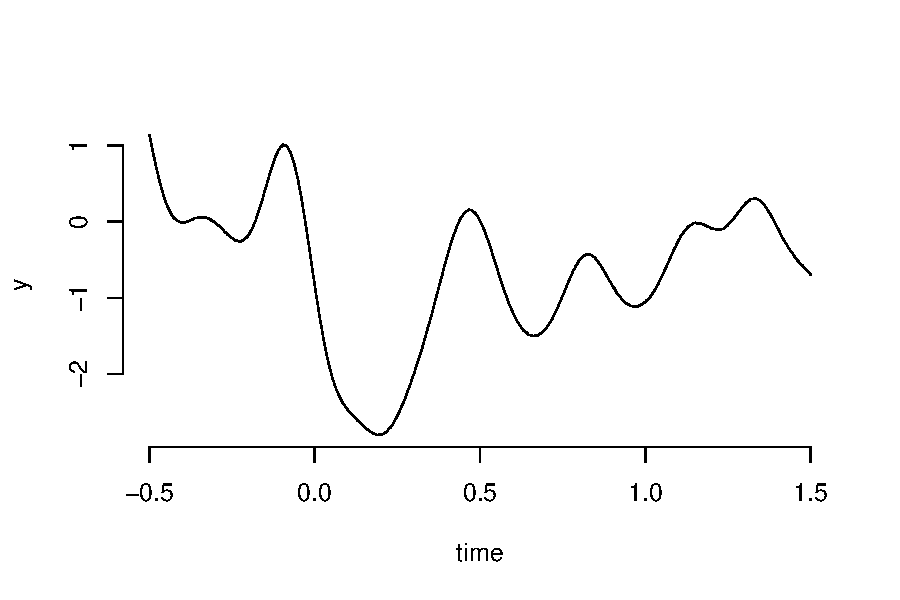
\includegraphics[width=\maxwidth]{figure/unnamed-chunk-4-1} 

}



\end{knitrout}

Notice that the {\tt chol()} produces an upper-right matrix. But as $U = L^T$ we transpose this using the transpose function {\tt t()}. Then we use {\tt \%*\%} for matrix multiplication.\\


%%%%%%%%%%%%%%%%%%%%%%%%%%%%%%%%%%%%%%%%%%%%%%%
\vspace{0.4cm}
\textbf{Using R functions}\\

The {\tt rmvnorm()} function (from the {\tt mvtnorm} package) creates random vectors with a single line. In fact it has three different methods to do this. The default uses the eigen-decomposition of the covariance matrix. But by setting {\tt method = "chol"} it will use the Cholesky approach explained above. 

There is another function, called {\tt mvrnorm()} (in the {\tt MASS} package\footnote{This is a `base' R package, meaning it is already installed}), which will produce random Gaussian vectors from a mean vector and covariance matrix. This uses the eigen-decomposition of the covariance matrix. 

Let's compare these three by making $m=200$ draws of an $n=1000$ vector.

\begin{knitrout}
\definecolor{shadecolor}{rgb}{0.969, 0.969, 0.969}\color{fgcolor}\begin{kframe}
\begin{alltt}
\hlstd{n} \hlkwb{<-} \hlnum{1000}
\hlstd{m} \hlkwb{<-} \hlnum{200}
\hlstd{t} \hlkwb{<-} \hlnum{1}\hlopt{:}\hlstd{n}
\hlstd{tau} \hlkwb{<-} \hlkwd{outer}\hlstd{(t, t,} \hlstr{"-"}\hlstd{)}  \hlcom{# compute t_j - t_i}
\hlstd{tau} \hlkwb{<-} \hlkwd{abs}\hlstd{(tau)}          \hlcom{# compute |t_j - t_i|}
\hlstd{S} \hlkwb{<-} \hlkwd{acv}\hlstd{(tau,} \hlnum{1.0}\hlstd{,} \hlnum{50}\hlstd{)}   \hlcom{# acf(tau) }

\hlcom{# add a small 'epsilon' value on diagonal}
\hlkwd{diag}\hlstd{(S)} \hlkwb{<-} \hlkwd{diag}\hlstd{(S)} \hlopt{+} \hlnum{0.0001}
\hlstd{mu} \hlkwb{<-} \hlkwd{rep}\hlstd{(}\hlnum{0}\hlstd{,} \hlnum{1000}\hlstd{)}       \hlcom{# mean values}

\hlcom{# compute the randon values, record the compute time}
\hlkwd{system.time}\hlstd{(}
  \hlstd{y} \hlkwb{<-} \hlstd{mvtnorm}\hlopt{::}\hlkwd{rmvnorm}\hlstd{(m,} \hlkwc{mean} \hlstd{= mu,} \hlkwc{sigma} \hlstd{= S)}
  \hlstd{)}
\end{alltt}
\begin{verbatim}
##    user  system elapsed 
##    2.29    0.04    2.42
\end{verbatim}
\end{kframe}
\end{knitrout}

This is the {\tt mvtnorm::rmvnorm} function, which by default uses the eigen-decomposition method. The output {\tt y} is an $m \times n$ vector, each row is one of the $n$-dimensional vectors.

We can also ask it to use the Cholesky method:

\begin{knitrout}
\definecolor{shadecolor}{rgb}{0.969, 0.969, 0.969}\color{fgcolor}\begin{kframe}
\begin{alltt}
\hlkwd{system.time}\hlstd{(}
  \hlstd{y} \hlkwb{<-} \hlstd{mvtnorm}\hlopt{::}\hlkwd{rmvnorm}\hlstd{(m,} \hlkwc{mean} \hlstd{= mu,} \hlkwc{sigma} \hlstd{= S,} \hlkwc{method} \hlstd{=} \hlstr{"chol"}\hlstd{)}
  \hlstd{)}
\end{alltt}
\begin{verbatim}
##    user  system elapsed 
##    0.39    0.05    0.43
\end{verbatim}
\end{kframe}
\end{knitrout}

Notice how this is much faster. There is a third method, using SVD (singular value decomposition).

\begin{knitrout}
\definecolor{shadecolor}{rgb}{0.969, 0.969, 0.969}\color{fgcolor}\begin{kframe}
\begin{alltt}
\hlkwd{system.time}\hlstd{(}
  \hlstd{y} \hlkwb{<-} \hlstd{mvtnorm}\hlopt{::}\hlkwd{rmvnorm}\hlstd{(m,} \hlkwc{mean} \hlstd{= mu,} \hlkwc{sigma} \hlstd{= S,} \hlkwc{method} \hlstd{=} \hlstr{"svd"}\hlstd{)}
  \hlstd{)}
\end{alltt}
\begin{verbatim}
##    user  system elapsed 
##    3.81    0.06    3.89
\end{verbatim}
\end{kframe}
\end{knitrout}

This is slower. How about the {\tt MASS::mvrnorm} function?

\begin{knitrout}
\definecolor{shadecolor}{rgb}{0.969, 0.969, 0.969}\color{fgcolor}\begin{kframe}
\begin{alltt}
\hlkwd{system.time}\hlstd{(}
  \hlstd{y} \hlkwb{<-} \hlstd{MASS}\hlopt{::}\hlkwd{mvrnorm}\hlstd{(m,} \hlkwc{mu} \hlstd{= mu,} \hlkwc{Sigma} \hlstd{= S)}
  \hlstd{)}
\end{alltt}
\begin{verbatim}
##    user  system elapsed 
##    2.21    0.03    2.25
\end{verbatim}
\end{kframe}
\end{knitrout}

Perhaps not surprisingly, this is similar to {\tt mvtnorm::rmvnorm} using the (default) eigen-decomposition method. But what about doing the Cholesky method ourselves?

\begin{knitrout}
\definecolor{shadecolor}{rgb}{0.969, 0.969, 0.969}\color{fgcolor}\begin{kframe}
\begin{alltt}
\hlstd{start} \hlkwb{<-} \hlkwd{proc.time}\hlstd{()}
\hlcom{# Cholesky decomposition of covariance matrix (n*n)}
  \hlstd{L} \hlkwb{<-} \hlkwd{t}\hlstd{(}\hlkwd{chol}\hlstd{(S))}
\hlcom{# generate n * m random numbers with Normal(0,1) distribution}
  \hlstd{X} \hlkwb{<-} \hlkwd{rnorm}\hlstd{(n}\hlopt{*}\hlstd{m,} \hlkwc{mean} \hlstd{=} \hlnum{0}\hlstd{,} \hlkwc{sd} \hlstd{=} \hlnum{1}\hlstd{)}
\hlcom{# re-shape these into an n * m matrix}
  \hlkwd{dim}\hlstd{(X)} \hlkwb{<-} \hlkwd{c}\hlstd{(n, m)}
\hlcom{# multiply n*n matrix L by n * m matrix X}
  \hlstd{y} \hlkwb{<-} \hlstd{L} \hlopt \hlstd{X}
\hlcom{# result is an n * m matrix. }
\hlstd{finish} \hlkwb{<-} \hlkwd{proc.time}\hlstd{()}
\hlkwd{print}\hlstd{(finish}\hlopt{-}\hlstd{start)}
\end{alltt}
\begin{verbatim}
##    user  system elapsed 
##    0.39    0.01    0.41
\end{verbatim}
\end{kframe}
\end{knitrout}

This is comparable to {\tt mvtnorm::rmvnorm} with the Cholesky method, and faster than the eigen-decomposition method. Also, the result is an $n \times m$ matrix, with each column is an $n$-dimensional vector (it's the transpose of the way that the other routines output the result).

If you look in the code for the {\tt MASS::mvrnorm} and {\tt mvtnorm::rmvnorm} functions -- both of which are written in R -- you will see there are many lines that 'check' the input data.

\begin{knitrout}
\definecolor{shadecolor}{rgb}{0.969, 0.969, 0.969}\color{fgcolor}\begin{kframe}
\begin{alltt}
\hlstd{MASS}\hlopt{::}\hlstd{mvrnorm}
\hlstd{mvtnorm}\hlopt{::}\hlstd{rmvnorm}
\end{alltt}
\end{kframe}
\end{knitrout}

These lines first check that the input mean and covariance matrix have the right dimensions ($n$ and $n \times n$), and that the covariance matrix is symmetric and positive semi-definite. These additional checks may slow down the R functions a little, but make them `safer' to use. 

There is some advice available on the internet (e.g. Stack Exchange) suggesting that when the covariance matrix in nearly singular the Cholesky method is not very stable, and that the eigen-decomposition method can be better, but the (slower) SVD method is most stable. So -- like with many numerical methods -- there is a trade-off between speed and stability.

\end{document}

